%%__________________________________________________________________||
\section{Introduction}
\label{sec:introduction}

Astronomical observations have determined that 27\% of our Universes
energy content is composed of an unknown form of matter - dark matter
(DM) - that is entirely different from normal matter that contributes
just 5\%. DM has yet been only observed via gravitational interactions
and its precise nature remains one of the most important discoveries
in fundamental physics.  Astrophysical measurements indicate that DM
consists of very weakly interacting particles at a scale potentially
accessible at the Large Hadron Collider (LHC). Of several
complementary detection approaches potential collider production
offers particularly good sensitivity at low DM masses and offers
complementary sensitivity at larger masses while not being subject to
astro-physical uncertainties. Collider searches are also largely
independent to the spin-structure of the interaction and can
probe interactions where the DM particles couple preferentially to heavy flavour quarks that might be suppressed
in direct or indirect DM searches.

The new energy frontier of the LHC during Run~2 provides a unique
opportunity to search for the generic pair production of weakly interacting massive particles (WIMPs). This Physics Analysis Summary presents an inclusive search for the pair production of WIMPs in hadronic final states with one or more energetic jets and
missing transverse momentum, performed in pp collisions at a
centre-of-mass energy $\sqrt{s} = 13\TeV$. The analysed data sample
corresponds to an integrated luminosity of $2.6 \pm 0.1
\fbinv$~\cite{lumi} collected by the Compact Muon Solenoid (CMS)
experiment. Previous iterations of this search have been performed in
pp collisions at $\sqrt{s} = 7$~\cite{RA1Paper, RA1Paper2011,
  RA1Paper2011FULL}, $8$~\cite{RA1Paper2012, RA1Parked}, and
$13\TeV$~\cite{RA1Paper2015}.

The search strategy is based around two key aspects in order to
achieve a robust, inclusive search capable of exploiting the potential
of the new LHC energy frontier under the challenging conditions of new
beam and detector configurations early in Run~2. First, multiple tight
selection criteria are employed to suppress multijet production, a
manifestation of quantum chromodynamics (QCD), to a negligible level
relative to all other SM background processes. Second, the
experimental acceptance to a potential signal is maximised through the
use of trigger conditions that maintain the same low thresholds
employed during Run~1.

The strategy is built around the use of the kinematic variable
\alphat~\cite{Randall:2008rw, RA1Paper}, which provides powerful
discrimination against multijet production. The \alphat variable is
constructed from jet-based quantities to provide robust discriminating
power between sources of genuine and misreconstructed missing
transverse momentum, making it suitable for early searches operating
at new energy and luminosity frontiers. The \alphat variable is
utilised as part of the trigger conditions, providing high performance
in terms of maintaining low thresholds for a given trigger
bandwidth. Further variables are also employed to discriminate against
multijet production and suppress this background process to a
negligible level. The $\Delta\phi^{*}_{\rm min}$~\cite{RA1Paper}
variable exploits azimuthal angular information and also provides
strong rejection power against multijet events, including rare
energetic events in which neutrinos carry a significant fraction of a
jet's energy due to semileptonic decays of heavy-flavour mesons.

%The search is devised around the kinematic variable
%\alphat~\cite{Randall:2008rw, RA1Paper} that provides powerful
%discrimination against multijet production, a manifestation of quantum
%chromodynamics (QCD), and adheres to an inclusive strategy with the
%aim of providing sensitivity to the widest possible range of SUSY
%models. The \alphat variable is constructed from jet-based quantities
%to provide robust discriminating power between sources of genuine and
%misreconstructed missing transverse momentum, making it suitable for early
%searches. A further variable that exploits azimuthal angular
%information, known as $\Delta\phi^{*}_{\rm min}$~\cite{RA1Paper}, is
%also employed to suppress QCD multijet production, including potential
%contributions from semileptonic heavy-flavour decays, to a negligible
%level.

The search is based on an examination of the number of reconstructed
jets per event, the number of these jets identified as originating
from bottom quarks, and the scalar and vector sums of transverse
momenta of these jets. 
%The search exploits the use of \mht templates derived from simulation,
%which are extensively validated in data control regions. 
%These discriminating variables provide sensitivity to the different
%production mechanisms of massive coloured sparticles at hadron
%colliders (\ie squark-squark, squark-gluino, and gluino-gluino),
%third-generation squark signatures, and a large range of mass
%splittings between the parent sparticle and the LSP,
%respectively. 
Interpretations of the result %are
\fixme{\it will be} provided in the parameter space of simplified
models that represent the
pair production of WIMPs, shown in Figures~\ref{fig:feyn} and \ref{fig:feyn1}.
For light flavour quark models, the spin-0 mediator is assumed to have yukawa coupling to the initial state partons so the loop is dominated by the top quark in an analogous way to the production of the Higgs boson. The coupling of the spin-0 and spin-1 mediators to the WIMPs is assumed to be unity, while the coupling of the spin-1 mediator to SM states is set to 0.25, following the recommendations of the ATLAS-CMS Dark Matter Forum. 

%to four quarks and two LSPs via off-shell squarks of light or heavy
%flavour, as illustrated in Fig.~\ref{fig:feyn}.

\begin{figure*}[thb]
\centering
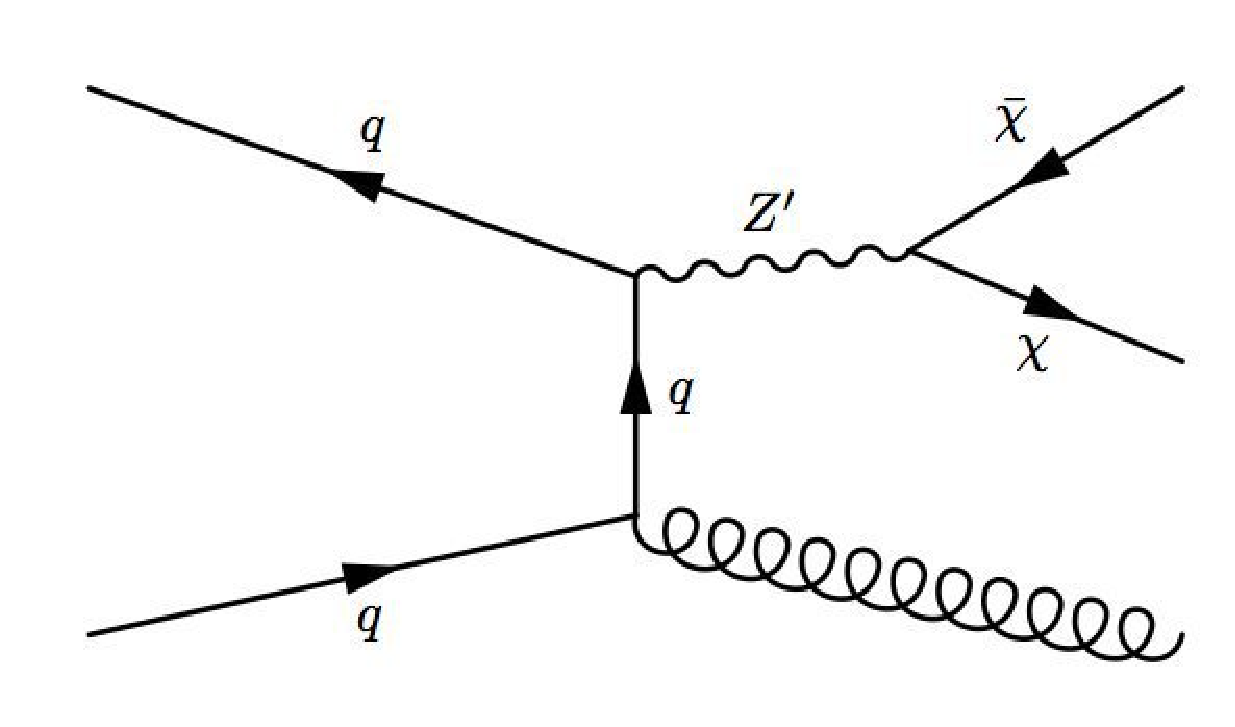
\includegraphics[width=0.35\linewidth]{vector.pdf}\,\,
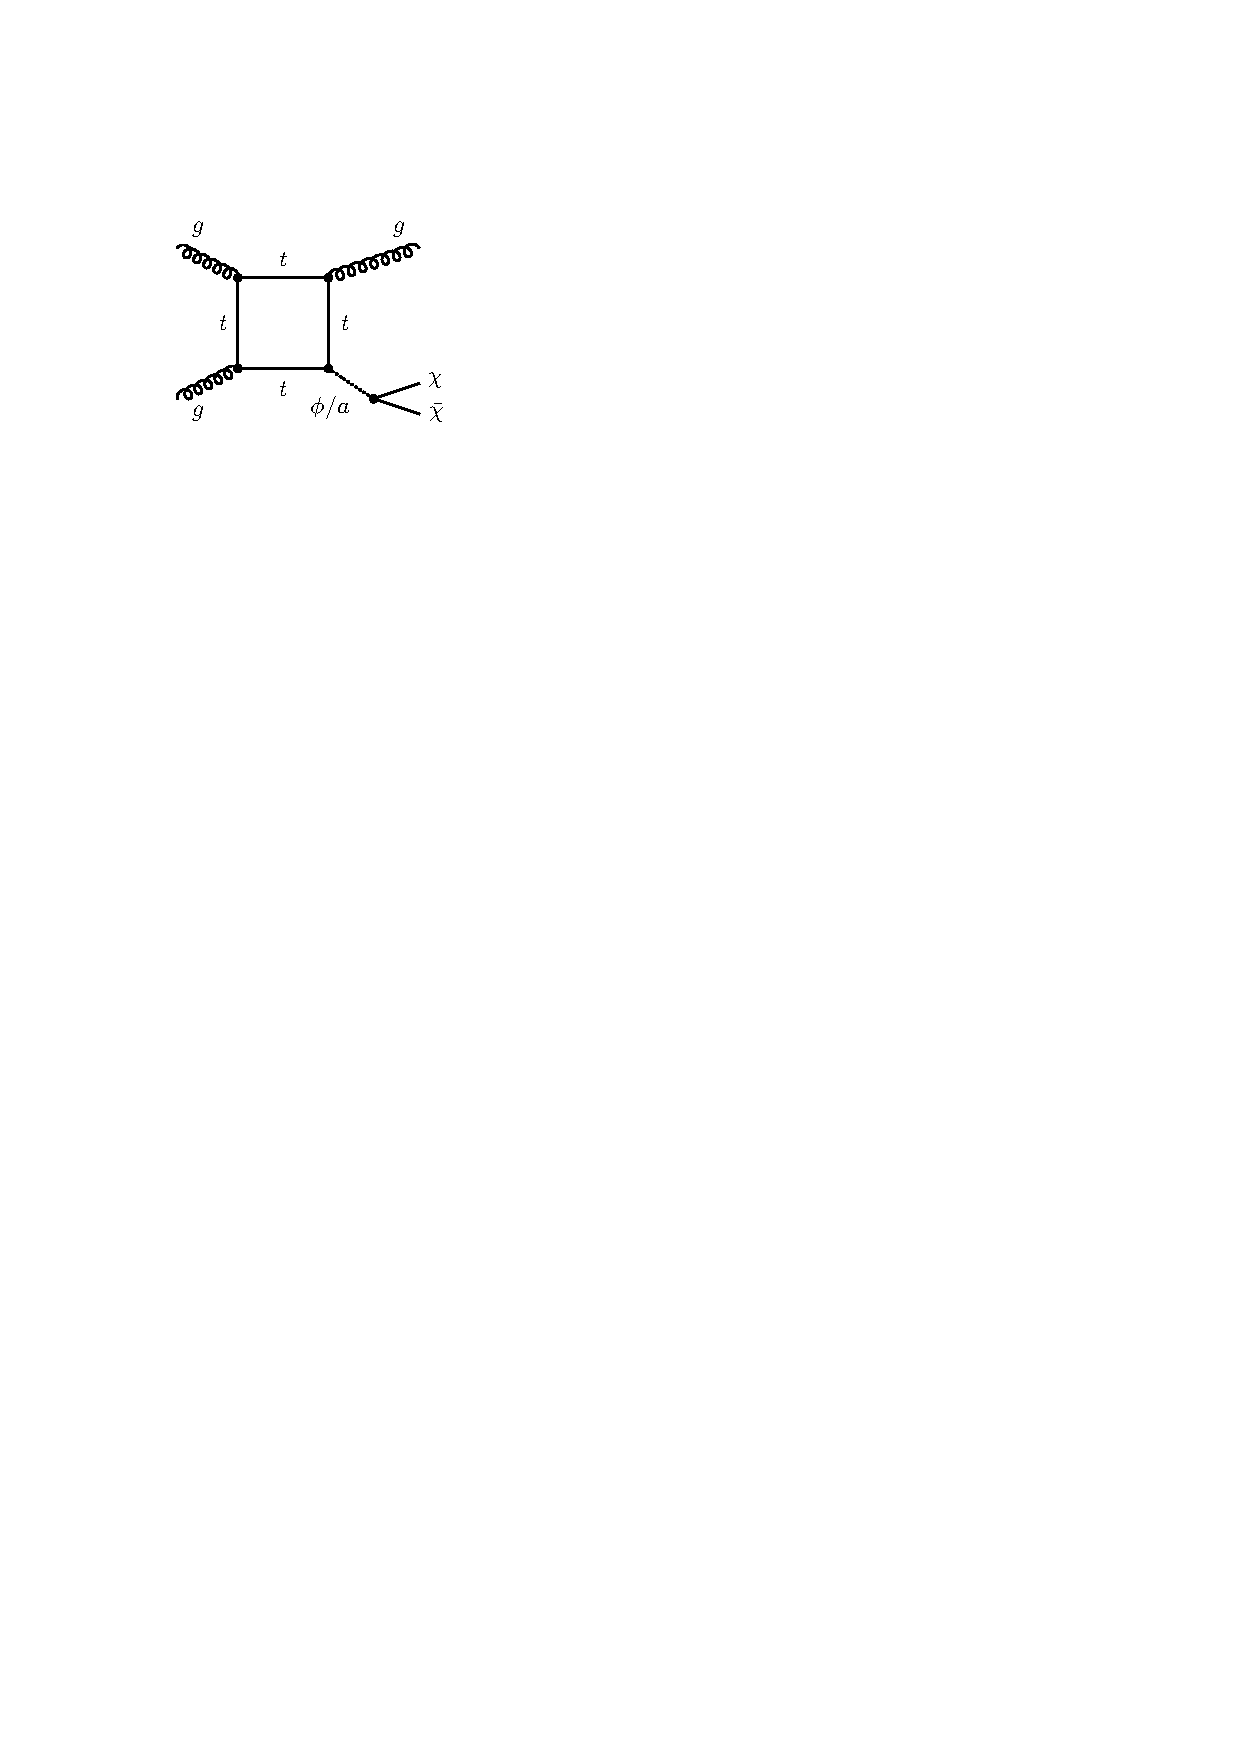
\includegraphics[width=0.35\linewidth]{scalar.pdf}
\caption{Representations of simplified models comprising the pair
  production of WIMPs in associated with jets from light flavour quarks for a (a) spin-1 mediator and (b) spin-0 mediator.}
\label{fig:feyn}
\end{figure*}

\begin{figure*}[thb]
\centering
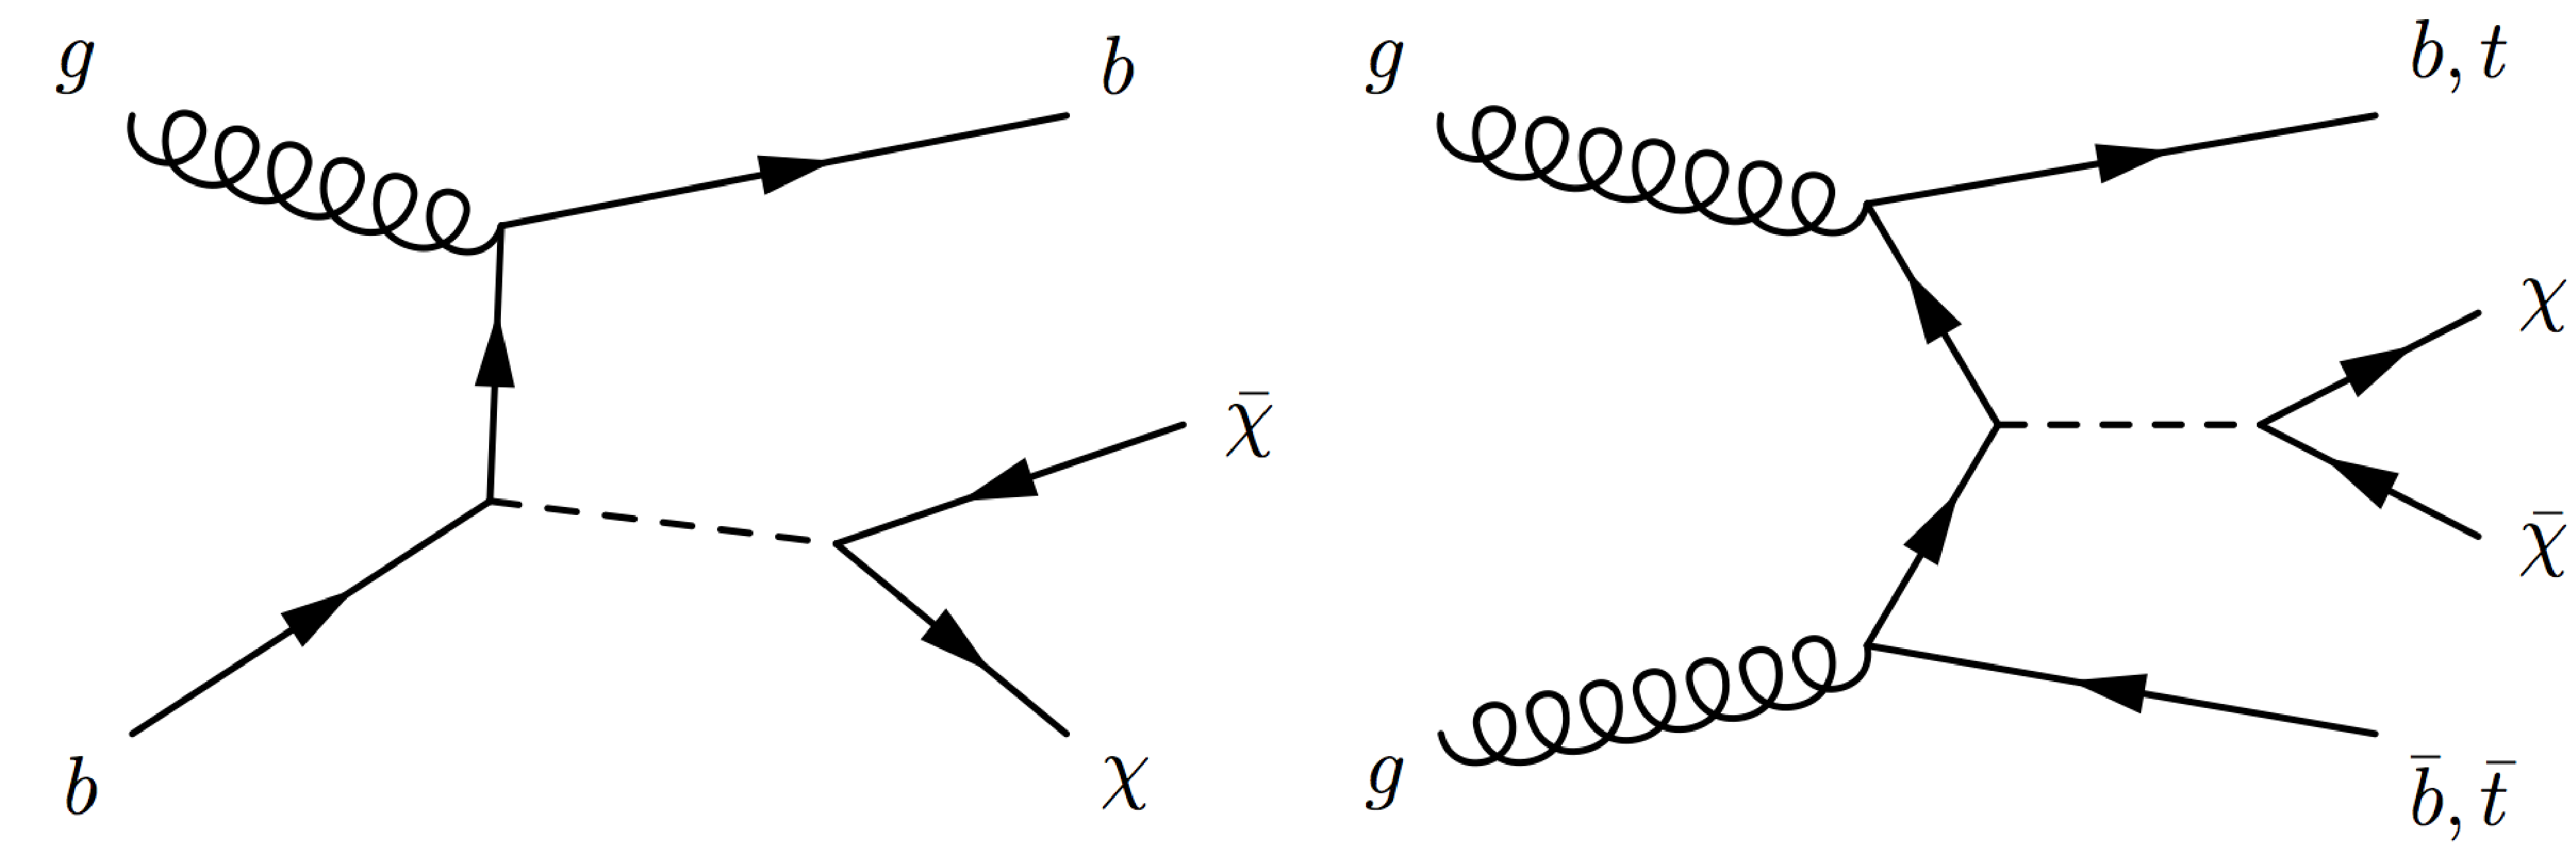
\includegraphics[width=0.65\linewidth]{feyn_heavy.pdf}
\caption{Representative feynman diagrams for simplified model comprising the pair production of WIMPs in association with jets from heavy flavour quarks for a spin-0 mediator.}
\label{fig:feyn1}
\end{figure*}


%%__________________________________________________________________||
